\section{Appendix}
\label{sec:Anhang}

\begin{table}
    \centering
    \sisetup{table-format = 1.2}
    \begin{tabular}{c c c c c}
        \toprule
 $t$ in $\si{\s}$ & $R_\text{recipient}$ in $\si{\ohm}$ 
 & $R_\text{shielding}$ in $\si{\ohm}$ & $I$ in $\si{\milli\A}$ &
 $U$ in $\si{\V}$ \\
        \midrule   
0	    & 27.3	& 25.5	 &  146.5	 & 15.36 \\	
374 	& 31.3	& 30.9	 &  147.8	 & 15.52 \\
779 	& 35.5	& 35.2	 &  148.3	 & 15.60 \\
1209	& 39.7	& 39.5	 &  148.8	 & 15.66 \\
1645	& 43.8	& 43.6	 &  149.1	 & 15.71 \\
2096	& 47.9	& 48.2	 &  149.3	 & 15.74 \\
2559	& 52.0	& 52.3	 &  149.5	 & 15.77 \\
3044	& 56.1	& 56.1	 &  149.7	 & 15.79 \\
3529	& 60.2	& 60.4	 &  149.8	 & 15.81 \\
4025	& 64.3	& 64.7	 &  149.9	 & 15.83 \\
4533	& 68.3	& 67.6	 &  149.9	 & 15.84 \\
5057	& 72.3	& 72.8	 &  150.0	 & 15.85 \\
5544	& 76.3	& 78.4	 &  150.1	 & 15.85 \\
6058	& 80.3	& 79.8	 &  150.1	 & 15.86 \\
6595	& 84.2	& 85.6	 &  150.2	 & 15.86 \\
7088	& 88.2	& 88.3	 &  150.2	 & 15.86 \\
7616	& 92.1	& 92.4	 &  150.2	 & 15.85 \\
8155	& 96.1	& 95.9	 &  150.3	 & 15.85 \\
8679	& 100.0	& 100.3	 &  150.3	 & 15.85 \\
9249	& 103.9	& 104.3	 &  150.3	 & 15.85 \\
9807	& 108.0	& 108.4	 &  150.4	 & 15.84 \\
        \bottomrule 
    \end{tabular}
    \caption{The measured data for $t$, $R_\text{recipient}$,$R_\text{shielding}$, $I$ and $U$.}
    \label{tab:Messwerte}
\end{table}

\begin{figure}
    \centering
    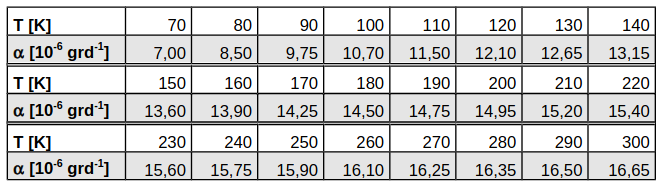
\includegraphics[width=\textwidth]{bilder/alpha.png}
   \caption{A table with the expansion coefficient dependent on the temperature \cite{V47}.}
   \label{tab:alpha}
\end{figure}


\begin{table}
    \centering
    \sisetup{table-format = 1.2}
    \begin{tabular}{c c c c c}
        \toprule
        $T$ in $\si{\kelvin}$ & $c_p$ in $\si{\joule\per\mole\kelvin}$ &  $c_v$ in $\si{\joule\per\mole\kelvin}$ \\
        \midrule   
        103,3  &  16,7838135837253  &  16,7838135836141 \pm 0,0000000000010  \\
        113,3  &  17,377181029556994  &  17,3771810294178 \pm 0,0000000000011  \\
        123,4  &  18,49597821808551  &  18,4959782179173 \pm 0,0000000000012  \\
        133,3  &  19,222473319255368  &  19,2224733190579 \pm 0,0000000000013  \\
        143,2  &  19,857871916586102  &  19,8578719163587 \pm 0,0000000000014  \\
        153,1  &  20,35997052466634  &  20,3599705244084 \pm 0,0000000000015  \\
        163,2  &  21,286754832458026  &  21,2867548321691 \pm 0,0000000000016  \\
        173,2  &  21,23237293759968  &  21,2323729372792 \pm 0,0000000000017  \\
        183,3  &  21,658849381967833  &  21,6588493816154 \pm 0,0000000000018  \\
        193,2  &  22,651958634209254  &  22,6519586338254 \pm 0,0000000000019  \\
        203,1  &  23,294803442144367  &  23,2948034417287 \pm 0,0000000000020  \\
        213,1  &  21,57129628265861  &  21,5712962822108 \pm 0,0000000000021  \\
        223,1  &  22,684145329655074  &  22,6841453291749 \pm 0,0000000000021  \\
        233,0  &  24,22073896202113  &  24,2207389615091 \pm 0,0000000000022  \\
        243,1  &  21,589446126860107  &  21,5894461263152 \pm 0,0000000000023  \\
        253,0  &  23,60122013215889  &  23,6012201315816 \pm 0,0000000000024  \\
        263,2  &  23,408576448683668  &  23,4085764480731 \pm 0,0000000000025  \\
        273,1  &  23,24408456452845  &  23,2440845638851 \pm 0,0000000000026  \\
        283,1  &  25,18173424453668  &  25,1817342438604 \pm 0,0000000000027  \\
        293,7  &  23,352435895537067  &  23,3524358948259 \pm 0,0000000000028  \\       
        \bottomrule 
    \end{tabular}
    \caption{The results for $c_p$ and $c_v$.}
    \label{tab:cv}
\end{table}

\begin{figure}
    \centering
    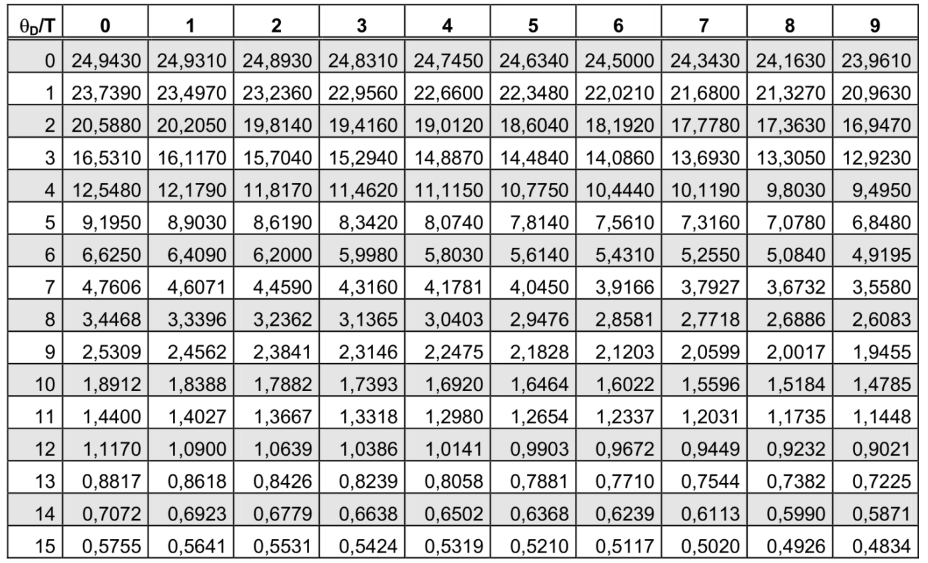
\includegraphics[width=\textwidth]{bilder/debye.png}
   \caption{A table with $\frac{\Theta_D}{T}$ dependent on  $c_v$ \cite{V47}.}
   \label{tab:deb}
\end{figure}